%==============================================================================
% Figure: Dimensional Folding Surface (2D -> 3D)
% Chapter: 13 - Origami Dimensions
% Data: dimensional_folding.json
%==============================================================================
% Purpose: Visualize fractal folding with golden ratio scaling showing
%          2D->3D dimensional progression via origami mechanism.
%          Z(x,y) = sum (A_n / phi^n) * sin(phi^n x) cos(phi^n y)
%==============================================================================

\begin{figure}[htbp]
  \centering

  % 2D cross-sections showing folding structure
  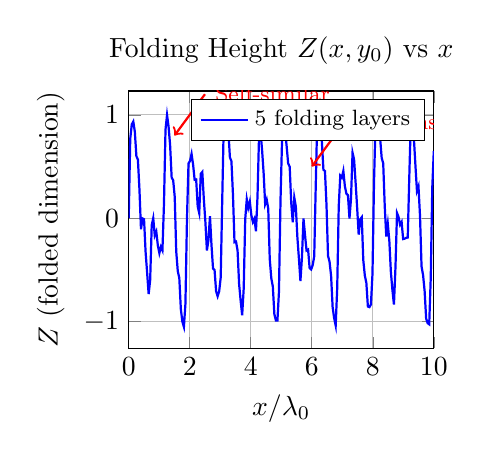
\begin{tikzpicture}
    \begin{axis}[
      width=0.45\textwidth,
      height=0.4\textwidth,
      title={Folding Height $Z(x, y_0)$ vs $x$},
      xlabel={$x / \lambda_0$},
      ylabel={$Z$ (folded dimension)},
      xmin=0, xmax=10,
      grid=major,
      legend pos=north east,
      legend style={font=\footnotesize},
    ]
    % Cross-section at y=5 (middle) - simplified representation
    % Golden ratio fractal folding pattern
    \addplot[
      blue, thick,
      domain=0:10,
      samples=200,
    ] {
      0.618*sin(deg(2*pi*x)) +
      0.382*sin(deg(2*pi*1.618*x)) +
      0.236*sin(deg(2*pi*1.618^2*x)) +
      0.146*sin(deg(2*pi*1.618^3*x)) +
      0.090*sin(deg(2*pi*1.618^4*x))
    };
    \addlegendentry{5 folding layers}

    % Show self-similarity at different scales
    \draw[<-, red, thick] (axis cs:1.5,0.8) -- (axis cs:2.5,1.2) node[right, font=\footnotesize] {Self-similar};
    \draw[<-, red, thick] (axis cs:6.0,0.5) -- (axis cs:7.0,0.9) node[right, font=\footnotesize] {patterns};
    \end{axis}
  \end{tikzpicture}%
  \hfill
  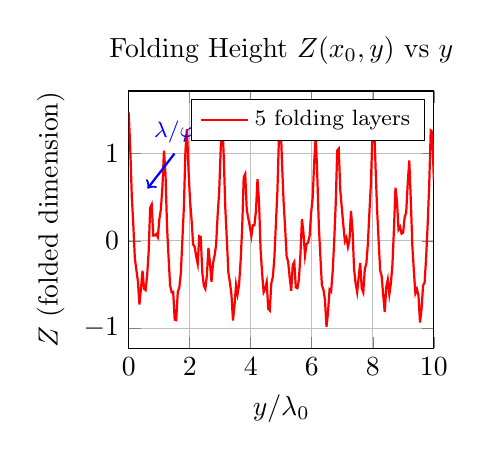
\begin{tikzpicture}
    \begin{axis}[
      width=0.45\textwidth,
      height=0.4\textwidth,
      title={Folding Height $Z(x_0, y)$ vs $y$},
      xlabel={$y / \lambda_0$},
      ylabel={$Z$ (folded dimension)},
      xmin=0, xmax=10,
      grid=major,
      legend pos=north east,
      legend style={font=\footnotesize},
    ]
    % Cross-section at x=5 (middle) with cosine modulation
    \addplot[
      red, thick,
      domain=0:10,
      samples=200,
    ] {
      0.618*cos(deg(2*pi*x)) +
      0.382*cos(deg(2*pi*1.618*x)) +
      0.236*cos(deg(2*pi*1.618^2*x)) +
      0.146*cos(deg(2*pi*1.618^3*x)) +
      0.090*cos(deg(2*pi*1.618^4*x))
    };
    \addlegendentry{5 folding layers}

    % Highlight golden ratio wavelengths
    \draw[<-, blue, thick] (axis cs:0.618,0.6) -- (axis cs:1.5,1.0) node[above, font=\footnotesize] {$\lambda/\varphi$};
    \end{axis}
  \end{tikzpicture}

  \vspace{0.3cm}

  % Conceptual 3D surface visualization
  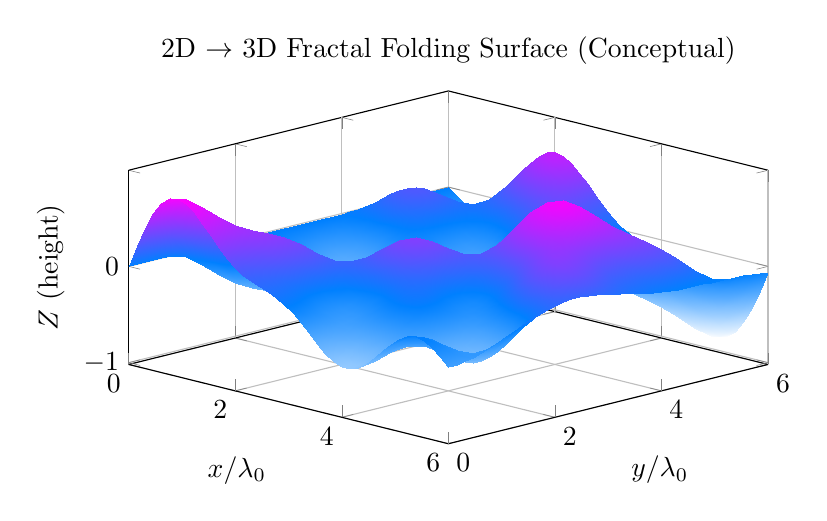
\begin{tikzpicture}
    \begin{axis}[
      width=0.8\textwidth,
      height=0.5\textwidth,
      title={2D $\to$ 3D Fractal Folding Surface (Conceptual)},
      xlabel={$x / \lambda_0$},
      ylabel={$y / \lambda_0$},
      zlabel={$Z$ (height)},
      view={45}{30},
      grid=major,
      colormap/cool,
      shader=interp,
    ]
    % 3D surface plot showing fractal folding
    \addplot3[
      surf,
      domain=0:6,
      domain y=0:6,
      samples=40,
      samples y=40,
    ] {
      0.5*sin(deg(x))*cos(deg(y)) +
      0.3*sin(deg(1.618*x))*cos(deg(1.618*y)) +
      0.2*sin(deg(1.618^2*x))*cos(deg(1.618^2*y))
    };
    \end{axis}
  \end{tikzpicture}

  \caption{%
    \textbf{Dimensional folding via origami mechanism with golden ratio scaling.}
    \textit{Top panels}: Cross-sections $Z(x, y_0)$ (left, blue) and $Z(x_0, y)$ (right, red)
    showing fractal self-similarity at multiple wavelengths $\lambda_0 / \varphi^n$
    where $\varphi = (1 + \sqrt{5})/2 = 1.618...$ is the golden ratio.
    Five folding layers superimpose with amplitudes $A_n = 1/n^2$ damping.
    \textit{Bottom}: Conceptual 3D surface $Z(x,y)$ demonstrating how 2D space (base plane)
    folds into 3D via
    $Z(x,y) = \sum_{n=1}^{5} (A_n / \varphi^n) \sin(\varphi^n x) \cos(\varphi^n y)$.
    This mechanism extends to 3D$\to$4D, 4D$\to$5D, enabling continuous fractal dimensions
    $d_H \approx 2.2$--2.4 in large-scale structure.
  }
  \label{fig:dimensional-folding}
\end{figure}

%==============================================================================
